\section{Previous Work}

Convolutional neural networks are designed to process pixelated data and discover visual patterns in the latent space. CNNs organize their data into three dimensions, the spatial dimensionality of the input (height and width) and the depth.

The CNN model is comprised of three types of layers following the input layer. A \textit{convolutional layer} uses a kernel filter in order to compute feature maps. The feature value of location $(i, j)$ in the $k$th feature map of the $i$th layer $z^l_{i, j, k'}$ is calculated by:
\begin{equation}
    z^l_{i, j, k} = w^{l^{T}}_kx^l_{i, j} + b^l_k
\end{equation}

where $w_k^l$ and $b_k^l$ are the weight vector and bias term of the $k$th filter at the $l$th layer. The activation function, usually sigmoid, tanh, or rectified lineur unit (ReLU), may then be calculated as:
\begin{equation}
    a^l_{i, j, k} = a(z^l_{i, j, k})
\end{equation}

A \textit{pooling} layer performs down-sampling along the spatial dimensionality of the given input in order to reduce dimensions. For each feature map $a^l_{i, j, k}$, pooling can be calculated as follows:
\begin{equation}
    y^l_{i, j, k} = pool(a^l_{m, n, k}), \forall(m, n) \in R_{ij}
\end{equation}

where $R_{ij}$ represents the local neighborhood around point $(i,j)$. Common pooling functions include max pooling and average pooling~\cite{gu2018recent}. Finally, \textit{fully-connected} layer takes input from the previous layer and connects them to neurons of the output layer in order to perform high-level reasoning or learn some global semantic information~\cite{OShea2015AnIT}.

LeNet~\cite{lenet} is a traditional CNN architecture for image recognition. It consists of two sets of convolutional, activation, and pooling layers. There is a final set of fully-connected, activation, and fully-connected layers with a softmax normalization and classification at the output layer.

Deep neural networks suffer from accuracy degradation due to how difficult it can become to map intermediary or residual layer outputs to inputs. A residual convolutional neural network (ResNet) is built up of blocks of stacked layers formed from a series of convolutions and non-linear activation functions. Following the authors who first introduced deep residual networks~\cite{resnet}, we define a block as:
\begin{equation}
    y = F(x, \{W_i\}) + x
\end{equation}

Where $x$ and $y$ are the input and output vectors, respectively, and $F(x, \{W_i\})$ is the residual mapping with a set of weights $W_i$. If $H(x)$ represents the ideal output mapping that corresponds to the ground truth, residual networks hypothesize that $F(x) + x = H(x)$. The residual function is pushed to zero such that the equation becomes an identity function $H(x) = x$. This identity mapping, or shortcut layer, is what reduces the degradation problem and minimizes training error as the network becomes deeper~\cite{resnet}.

CNNs have been used to classify network traffic in multiple problems for both per-packet and per-flow scenarios. Lim et al~\cite{lim2019network} also transform packets into grayscale images and label them by application (RDP, Skype, BitTorrent, and others). They use both a CNN and ResNet architecture. When using payloads of 1024B and a ResNet architecture, they achieved a 0.97 F1 score for accurately classifying the packets as one of eight types of applications.

Yang et al~\cite{yang2022} use quantile normalization to transform network packets in CANs into pixelated images for CNN processing. They also take a flow-based strategy, combining multiple packets into a single image. For example, they propose taking 27 packets with 9 features each and creating a $9 \times 9 \times 3$ image, where three channels RGB (red, green, blue) are provided for a single pixel. This is then used as input into their CNN architecture.

Similarly, Gao~\cite{Gao2022} proposes a CNN-LSTM architecture which reduces false positive rates in his network intrusion detection system for cloud computing environments. Numerical and character attributes from the KDD CUP 99 test data set are first pre-processed into a $10 \times 42$ matrix, where window size $w = 10$ and the number of features in the data set is 42. The data set is transposed to an image dataset where each matrix $W$ is mapped to a $10 \times 42$ grayscale image. If $v_{ij}$ represents the value of a pixel in matrix/image $W$ at position $i,j$, the values $v_{ij} \in [0,255]$. To reduce the data interval and normalize values, the following formula is used:
\begin{equation}
    x = \frac{x-\overline{x}}{\delta}
\end{equation}

where $x$ is the current value of a certain data in the sequence, $\overline{x}$ is the mean value of the data in the series, and $\delta$ is the standard deviation of the sequence. Finally, this system adds an additional attention mechanism layer to improve classification accuracy:
\begin{equation}
    \begin{split}
    u_t = tanh(W_wP_t + b_w), \\
    a_t softmax(u_t^T, u_w), \\
    v = \sum a_tP-T,
    \end{split}
\end{equation}

where $u_t$ is the attribute representation of $P_t$, $W_w$ is the context vector randomly generated during training, $a_t$ is the importance weight, and $v$ is the high-level representation obtained through importance weight summation on $P_t$. \\

Jo et al~\cite{jo2020packet} use a CNN-LSTM hybrid model to perform network intrusion detection, but first pre-process packets into image representations. Namely, they adapt the NSL-KDD dataset which has 41 fields into pixel representations. Continuous fields are first normalized to a $[0-255]$ range to create a grayscale image pixel value. Symbolic fields such as ``protocol type" are represented by the same kind of pixel value, but normalized based on the number of possibilities. For example, a symbolic value with three possibilities will be normalized as 0, 128, or 255~\cite{jo2020packet}. $28 \times 28$ images are created and processed with a $5 \times 5$ kernel as shown in Figure~\ref{fig:kernel}.

\begin{figure} [h!]
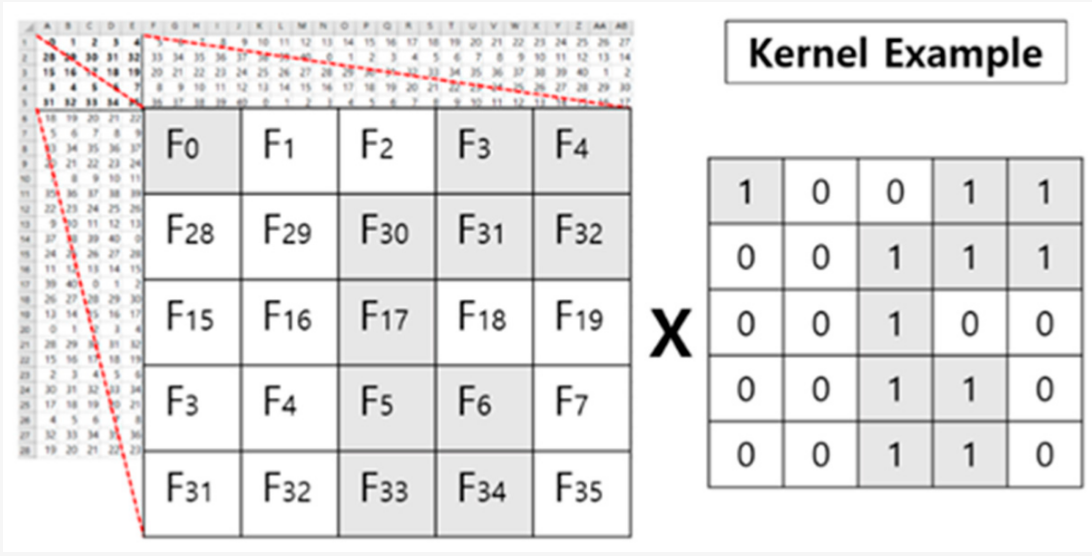
\includegraphics[width=\linewidth]{chapters/5/img/kernel.png}
\caption{Example application of kernel to pixelated packet data~\cite{jo2020packet}}
\label{fig:kernel}
\end{figure}

Deep Packet~\cite{lotfollahi2020deep} is a well-cited work in deep learning for traffic classification. They use a stacked auto-encoder and CNN to perform traffic classification into traffic types and application types as labeled in the VPN/non-VPN UNB ISCX dataset~\cite{vpn-dataset}. Their solution achieves 94\% accuracy in the traffic classification task per traffic type, and 97\% accuracy in the application classification task. Incorporating the same dataset as well as additional, more recent flows, we are able to achieve higher accuracy in RTP detection with a less computationally complex framework in \textsc{Maple}.
